\documentclass{jsarticle}
\usepackage{changepage,amsmath,amssymb,ascmac}
\usepackage[dvipdfmx]{graphicx}
\newenvironment{indentblock}{\begin{adjustwidth}{\parindent}{}\hspace{-\parindent}}{\end{adjustwidth}}

\begin{document}

まず、$3^2=9$という簡単な式を考えます。
$3 \times 3=9$(3を2回かけたら9)という意味になりますが、これをlogを使って表すとこうなります。
\[\log_3 9=2\]
$\log$のgの下に小さく書いてある数字(=3)を9にするためには2回かければいいってことになります。\\

まとめるとこうなります\\
\[a^b=c ならば \log_a c=b\]
\[例:5^3=125 ならば \log_5 125=3\]
\hrulefill

問題9の(1)を見てみます。\\
\[256=2^n\]
これは2をn回かけたら256という意味なので
\[\log_2 256=n\]
となります。
もしくは、\[a^b=c ならば \log_a c=b\]を公式のようにみてみれば同じ答えになります。
(2)や(3)も同じ要領で解くことができます。\\
\dotfill

(2)は32を$\frac{1}{5}$回かけたら2って意味なので、
\[\log_32 2=\frac{1}{5}\]となります。\\
\dotfill

(3)は4を-3回かけたら$\frac{1}{64}$になるってことなので、
\[\log_4 \frac{1}{64}=-3\]となります。\\
\hrulefill

問題10は、ちょうど問題9の逆です。\\
(1)\par
$\log_10 100=2$の意味するところは10を2乗したら100になったということですので、こうなります。\\
\[10^2=100\]
\dotfill

(2), (3), (4)\par
(1)と同様に考えて、\\
\begin{indentblock}\\
(2)$6^{-2}=\frac{1}{36}$\\
(3)$4^{\frac{3}{2}}=8$\\
(4)$\frac{1}{6}^{-2}=36$\\
\end{indentblock}
となります。\\
\hrulefill\\
問題11は、書き換えではなく計算になりますが、上がわかればそこまで難しくありません。\\
(1)
\begin{indentblock}
$\log_6 36$というのは、「6を何回かかけ合わせたら36になりますか?」ということです。\\
$6 \times 6=6^2=36$なので2回かけ合わせれば36になります。\\
$\therefore$ 答えは2になります。
\end{indentblock}
\dotfill\\
(2), (3), (4), (5), (6)\par
いずれも(1)と同様に解きます。
\begin{indentblock}
(2) $4^3=64$なので3\\
(3) $8^{-1}=\frac{1}{8}$なので-1\\
(4) $10^{-2}=\frac{1}{100}$なので-2\\
(5) $7^{\frac{1}{2}}=\sqrt{7}$なので$\frac{1}{2}$\\
(6) $6^{\frac{1}{3}}=\sqrt[3]{6}$なので$\frac{1}{3}$\\
となります。
\end{indentblock}
\begin{itembox}[l]{指数に分数とかマイナスの数とかついてるときの計算}
$a^{\frac{1}{b}}=\sqrt[b]{a}$\\
$a^{-b}=\frac{1}{a^b}$\\
なので\\
$a^{\frac{b}{c}}=a^{b\times \frac{1}{c}}=(a^b)^{\frac{1}{c}}=\sqrt[c]{a^b}$\\
となります。
\end{itembox}\\
\hrulefill\\
$\log$のgの下にくっついてる数を底といいます。底が同じ$\log$どうしの足し算、引き算では次の公式が使えます。\\
\begin{itembox}[l]{底が同じ$\log$どうしの足し算・引き算}
$\log_a b+\log_a c=log_a b\times c$\\
$\log_a b-\log_a c=log_a \frac{b}{c}$\\
$\log$の外の足し算は$\log$の中では掛け算に\\
$\log$の中の引き算は$\log$の中では割り算に\\
\end{itembox}
これを使って問題12を解けます。\\
(1) $\log_6 12+\log_6 3=\log_6 12\times 3=\log_6 36=\log_6 6^2=2$\\
(2) $\log_{10} 25+\log_{10} 4=\log_{10} 25\times 4=\log_{10} 100=\log_{10} 10^2=2$\\
足し算は掛け算になります。\\
(3) $\log_3 75-\log_3 25=\log_3 \frac{75}{25}=\log_3 3=1$\\
(4) $\log_2 56-\log_2 14=\log_2 \frac{56}{14}=\log_2 4=\log_2 2^2=2$\\
引き算は割り算になります。
%
% ページ区切り
\newpage
%
\begin{itembox}[l]{$\log$の単調性}
$\log_a x$のとき、$x$が大きければ大きいほど、$\log_a x$も大きくなります。\\
逆に、$x$が小さければ小さいほど、$\log_a x$も小さくなります。\\
たとえば、$\log_3 10$と$\log_3 20$は、中身がそれぞれ10、20なので、$\log_3 10<\log_3 20$となります。
\end{itembox}
つまり、$\log$のついていない数も$\log$に直してから、$\log$の中身を比較すればよいことになります。\\
\begin{itembox}[l]{$\log$と数の掛け算}
次の式が成り立ちます。\\
$a\log_b c=\log_b c^a$\\
たとえば、
$5\log_2 7=\log_2 7^5$\\
となります。
\end{itembox}
問題14\\
(1)
\begin{indentblock}
0以外は底が2なので、それぞれの数を$\log_2$の式に変形していきます。\\
\[2\log_2 3=\log_2 3^2=\log_2 9\]
\[3\log_2 2=\log_2 2^3=\log_2 8\]
また、2はどんなに少ない回数かけても、0には絶対なりませんので、
\[0<\log_2 8<\log_2 9\]
となります。元の形に戻すと、
\[0<3\log_2 2<2\log_2 3\]
となります。
\end{indentblock}
\dotfill\\
(2)
\begin{indentblock}
底がすべて同じなので、それぞれを$\log$の式に変形していきます。\\
\[2\log_{\frac{1}{3}} 5=\log_{\frac{1}{3}} 5^2=\log_{\frac{1}{3}} 25\]
\[3\log_{\frac{1}{3}} 4=\log_{\frac{1}{3}} 4^3=\log_{\frac{1}{3}} 64\]
\[4\log_{\frac{1}{3}} 3=\log_{\frac{1}{3}} 3^4=\log_{\frac{1}{3}} 81\]
なので、logの中身を比較して、
\[\log_{\frac{1}{3}} 25<\log_{\frac{1}{3}} 64< \log_{\frac{1}{3}} 81\]
となります。元の形に戻すと、
\[2\log_{\frac{1}{3}} 5<3\log_{\frac{1}{3}} 4<4\log_{\frac{1}{3}} 3\]
となります。
\end{indentblock}
\dotfill\\
(3)
\begin{indentblock}
(2)と同様、底がすべて同じなので、それぞれを$\log$の式に変形していきます。\\
\[2\log_3 2=\log_3 2^2=\log_3 4\]
\[4\log_3 \sqrt{3}=4\log_3 3^{\frac{1}{2}}=\log_3 3^{\frac{1}{2}\times 4}=\log_3 3^2=\log_3 9\]
\[3\log_3 2=\log_3 2^3=\log_3 8\]
なので、logの中身を比較して、
\[\log_3 4<\log_3 8<\log_3 9\]
となるので、元の形に戻すと、
\[2\log_3 2<3\log_3 2<4\log_3 \sqrt{3}\]
となります。
\end{indentblock}
\dotfill\\
(4)
\begin{indentblock}
(2)と同様、底がすべて同じなので、それぞれを$\log$の式に変形していきます。\\
\[4\log_{\frac{1}{2}} 3=\log_{\frac{1}{2}} 3^4=\log_{\frac{1}{2}} 81\]
\[2\log_{\frac{1}{2}} 7=\log_{\frac{1}{2}} 7^2=\log_{\frac{1}{2}} 49\]
\[6\log_{\frac{1}{2}} 2=\log_{\frac{1}{2}} 2^6=\log_{\frac{1}{2}} 64\]
なので、logの中身を比較して、
\[\log_{\frac{1}{2}} 49<\log_{\frac{1}{2}} 64<\log_{\frac{1}{2}} 81\]
となるので、元の形に戻すと、
\[2\log_{\frac{1}{2}} 7<6\log_{\frac{1}{2}} 2<4\log_{\frac{1}{2}} 3\]
となります。
\end{indentblock}
\hrulefill\\
\begin{itembox}[l]{平均変化率}
平均変化率は、関数上の2点を結んだとき、その直線の傾きを言います。\\
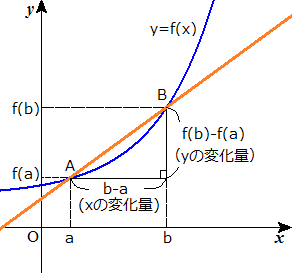
\includegraphics{20150726230645b0e.png}\\
\small{(http://highmath.blog.fc2.com/blog-entry-70.htmlからの引用)}\\
$x$が$a$から$b$まで変化するときの平均変化率は、式で書くとこうなります。\\
\[(平均変化率)=\frac{f(b)-f(a)}{b-a}\]
\end{itembox}
問題15\\
(1)
\begin{indentblock}
\[(平均変化率)=\frac{f(3)-f(2)}{3-2}=3^2-2^2=9-4=5\]
\end{indentblock}
\dotfill\\
(2)
\begin{indentblock}
\[(平均変化率)=\frac{f(4)-f(-1)}{4-(-1)}=\frac{4^2-(-1)^2}{5}=\frac{16-1}{5}=3\]
\end{indentblock}
\dotfill\\
(3)
\begin{indentblock}
\[(平均変化率)=\frac{f(1+h)-f(1)}{1+h-1}=\frac{\{-(1+h)^2\}-(-1^2)}{h}=\frac{\{-(1+2h+h^2)\}+1}{h}=\frac{-2h-h^2}{h}=-2-h\]
\end{indentblock}
\hrulefill\\
\begin{itembox}[l]{極限値の求め方}
$\lim$とは、例えば、$\displaystyle \lim_{x \to a} f(x)$のとき、$f(x)$の$x$を$a$に限りなく近づけること。\\
$\rightarrow$ $\displaystyle \lim_{x \to 5} x$であればxに5を代入したものと同じ0になる。\\
$\rightarrow$ $\displaystyle \lim_{x \to 5} \frac{h^2}{h}$であれば、0を直接代入すると、$\frac{0}{0}$となってしまうが、$\displaystyle \lim_{x \to 0} \frac{h^2}{h}=\lim_{x \to 0} h$と約分して分母の0を解消すれば答えは5とわかる。
このように、そのまま代入して答えが出れば代入し、($\frac{0}{0}$のようになって)答えが出なければ、変形して解消する。
\end{itembox}
問題16\\
(1)
\begin{indentblock}
$\displaystyle \lim_{h \to 0}(1-3h)=1$\\
(そのままhに0を代入したものと同じ)
\end{indentblock}
\dotfill\\
(2)
\begin{indentblock}
$\displaystyle \lim_{h \to 0}(16-8h+h^2)=16$\\
(そのままhに0を代入したものと同じ)
\end{indentblock}
\dotfill\\
(3)
\begin{indentblock}
$\displaystyle \lim_{h \to 0}\frac{h+h^2}{h}=\lim_{h \to 0}(1+h)=1$\\
(そのままhに0を代入すると$\frac{0}{0}$となってしまうので、約分して分母が0にならないようにする)
\end{indentblock}
\dotfill\\
(4)
\begin{indentblock}
$\displaystyle \lim_{h \to 0}\frac{-2h+h^2}{h}=\lim_{h \to 0}(-2+h)=-2$\\
(そのままhに0を代入すると$\frac{0}{0}$となってしまうので、約分して分母が0にならないようにする)
\end{indentblock}
\hrulefill\\
\begin{itembox}[l]{微分公式}
\begin{enumerate}
\item $y$を微分したものを$y'$と書きます。
\item $x^a$を微分すると$ax^{a-1}$となります。\\
例えば、$x^5$を微分すると$5x^4$となります。
\item 足し算や引き算の式を微分するときは、微分したものを足し(引き)ます。\\
例えば、$x^2+x$を微分すると$2x+1$となります。\\
($x$は$x^1$と考えます)
\end{enumerate}
\end{itembox}
問題17\\
(1)
\begin{indentblock}
$y'=5\times 2x^{2-1}=10x$
\end{indentblock}
\dotfill\\
(2)
\begin{indentblock}
$y'=-3\times 3x^2=-9x^2$
\end{indentblock}
\dotfill\\
(3)
\begin{indentblock}
$y'=0$
(yはxに関係なく常に7となる。$y=x^0+0$と考えるといいかも)
\end{indentblock}
\dotfill\\
(4)
\begin{indentblock}
$y'=5\times 2x-3\times 1x^0=10x-3$
\end{indentblock}
\dotfill\\
(5)
\begin{indentblock}
$y'=\frac{1}{3}\times 3x^2+2x=x^2+2x$
\end{indentblock}
\dotfill\\
(6)
\begin{indentblock}
$y'=-2\times 3x^2+4\times 2x=-6x^2+8x$
\end{indentblock}
\dotfill\\
(7)
\begin{indentblock}
$y=(x+1)(x-1)=x^2-1$\\
$y'=2x$
\end{indentblock}
\dotfill\\
(8)
\begin{indentblock}
$y=4x^2-4x+1$\\
$y'=4\times 2x-4=8x-4$
\end{indentblock}
\hrulefill\\
こんな感じです。最後のほうの微分は指数を前にくっつけて、元の指数から1引くイメージです!\\
説明へたくそなんでなにかあったら質問ください。よろしくおねがいしますね!
\end{document}

